\documentclass{beamer}
\usepackage{graphicx} % Required for inserting images

\usepackage{amsmath}
\usepackage{amssymb}
\usepackage{amsfonts}
\usepackage{amsthm}
\usepackage{tikz}
\usepackage{tabularx}
\usepackage{multirow}
\usepackage[sorting=none, style=ieee, block=ragged]{biblatex}
\usepackage{pgfplots}
\pgfplotsset{compat=1.17}
\usetikzlibrary{matrix, positioning, arrows}


% set theme
\usetheme{Berlin}
\usecolortheme{beaver}

\makeatother
\setbeamertemplate{footline}
{
  \leavevmode%
  \hbox{%
  \begin{beamercolorbox}[wd=.4\paperwidth,ht=2.25ex,dp=1ex,center]{author in head/foot}%
    \usebeamerfont{author in head/foot}\insertshortauthor
  \end{beamercolorbox}%
  \begin{beamercolorbox}[wd=.6\paperwidth,ht=2.25ex,dp=1ex,center]{title in head/foot}%
    \usebeamerfont{title in head/foot}\insertshorttitle\hspace*{3em}
    \insertframenumber{} / \inserttotalframenumber\hspace*{1ex}
  \end{beamercolorbox}}%
  \vskip0pt%
}
\makeatletter
\setbeamertemplate{navigation symbols}{}

% title
\title{Autoencoder Neural Networks for Digital Cryptography}
\author{Jaime Tenorio}
\date{
    Óbuda University \\
    John von Neumann Faculty of Informatics \\
    Information and Coding Theory \\
    Dr. Márta Takács \\
    May 2023
}

% references
\addbibresource{bib/references.bib}

\begin{document}

\maketitle

\begin{frame}
    \frametitle{Introduction}
    \begin{itemize}
        \item Cryptography is the study of techniques for secure communication.
        \item An encryption algorithm transforms a message into one that is difficult to predict or duplicate.
        \item The most popular and widely used involve the use of a key, like Advanced Encryption Standard (AES) \cite{aes}.
    \end{itemize}
    \centering
    \includegraphics[width=0.5\textwidth]{img/cryptodiagram.jpeg}
\end{frame}

\begin{frame}
    \frametitle{Introduction}
    \begin{itemize}
        \item Autoencoders are neural networks whose that learn efficient representations of data by unsupervised training \cite{autoencoder}.
        \item The network learns to encode the information in a latent space, capturing the essential features.
        \item Symmetric architecture -- the input has the same shape as the output. The middle layer is the code layer.
        \item Useful for dimensionality reduction, anomaly detection, signal processing, data compression, and cryptography.
    \end{itemize}
    \begin{equation}\label{eq:autoencoder}
        \begin{split}
            z &= g(x) \\
            x' &= f(z) \\
            x &\approx x' \\
        \end{split}
    \end{equation}
\end{frame}

\begin{frame}
    \frametitle{Introduction}
    \centering
    

\tikzset{every picture/.style={line width=0.75pt}} %set default line width to 0.75pt        

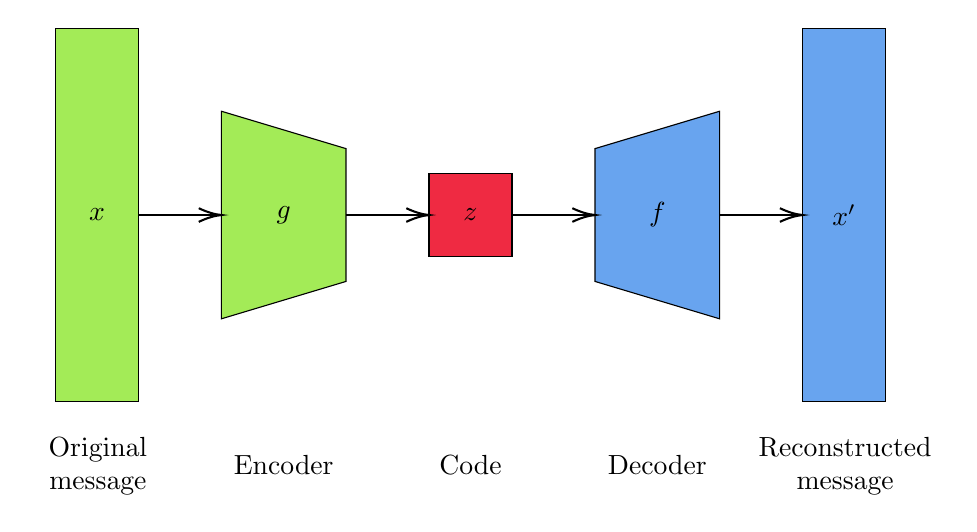
\begin{tikzpicture}[x=0.75pt,y=0.75pt,yscale=-1,xscale=1]
    %uncomment if require: \path (0,300); %set diagram left start at 0, and has height of 300

    %Shape: Rectangle [id:dp8942019960286618] 
    \draw  [fill={rgb, 255:red, 163; green, 235; blue, 87 }  ,fill opacity=1 ] (20,20) -- (60,20) -- (60,200) -- (20,200) -- cycle ;
    %Shape: Trapezoid [id:dp4630434446283549] 
    \draw  [fill={rgb, 255:red, 163; green, 235; blue, 87 }  ,fill opacity=1 ] (100,60) -- (160,78) -- (160,142) -- (100,160) -- cycle ;
    %Shape: Rectangle [id:dp7342042996288556] 
    \draw  [fill={rgb, 255:red, 239; green, 42; blue, 66 }  ,fill opacity=1 ] (200,90) -- (240,90) -- (240,130) -- (200,130) -- cycle ;
    %Shape: Trapezoid [id:dp8342225116725475] 
    \draw  [fill={rgb, 255:red, 104; green, 164; blue, 239 }  ,fill opacity=1 ] (340,60) -- (280,78) -- (280,142) -- (340,160) -- cycle ;
    %Shape: Rectangle [id:dp23031828799634058] 
    \draw  [fill={rgb, 255:red, 104; green, 164; blue, 239 }  ,fill opacity=1 ] (380,20) -- (420,20) -- (420,200) -- (380,200) -- cycle ;
    %Straight Lines [id:da7729793473503881] 
    \draw    (60,110) -- (98,110) ;
    \draw [shift={(100,110)}, rotate = 180] [color={rgb, 255:red, 0; green, 0; blue, 0 }  ][line width=0.75]    (10.93,-3.29) .. controls (6.95,-1.4) and (3.31,-0.3) .. (0,0) .. controls (3.31,0.3) and (6.95,1.4) .. (10.93,3.29)   ;
    %Straight Lines [id:da237260655681939] 
    \draw    (160,110) -- (198,110) ;
    \draw [shift={(200,110)}, rotate = 180] [color={rgb, 255:red, 0; green, 0; blue, 0 }  ][line width=0.75]    (10.93,-3.29) .. controls (6.95,-1.4) and (3.31,-0.3) .. (0,0) .. controls (3.31,0.3) and (6.95,1.4) .. (10.93,3.29)   ;
    %Straight Lines [id:da21321769920852573] 
    \draw    (240,110) -- (278,110) ;
    \draw [shift={(280,110)}, rotate = 180] [color={rgb, 255:red, 0; green, 0; blue, 0 }  ][line width=0.75]    (10.93,-3.29) .. controls (6.95,-1.4) and (3.31,-0.3) .. (0,0) .. controls (3.31,0.3) and (6.95,1.4) .. (10.93,3.29)   ;
    %Straight Lines [id:da5140682018274638] 
    \draw    (340,110) -- (378,110) ;
    \draw [shift={(380,110)}, rotate = 180] [color={rgb, 255:red, 0; green, 0; blue, 0 }  ][line width=0.75]    (10.93,-3.29) .. controls (6.95,-1.4) and (3.31,-0.3) .. (0,0) .. controls (3.31,0.3) and (6.95,1.4) .. (10.93,3.29)   ;

    % Text Node
    \draw (40.5,231) node   [align=left] {\begin{minipage}[lt]{44.12pt}\setlength\topsep{0pt}
            \begin{center}
                Original\\message
            \end{center}

        \end{minipage}};
    % Text Node
    \draw (400.5,231) node   [align=left] {\begin{minipage}[lt]{68.49pt}\setlength\topsep{0pt}
            \begin{center}
                Reconstructed\\message
            \end{center}

        \end{minipage}};
    % Text Node
    \draw (130,230.5) node   [align=left] {\begin{minipage}[lt]{40.72pt}\setlength\topsep{0pt}
            \begin{center}
                Encoder
            \end{center}

        \end{minipage}};
    % Text Node
    \draw (310,230.5) node   [align=left] {\begin{minipage}[lt]{41.28pt}\setlength\topsep{0pt}
            \begin{center}
                Decoder
            \end{center}

        \end{minipage}};
    % Text Node
    \draw (220,230.5) node   [align=left] {\begin{minipage}[lt]{27.1pt}\setlength\topsep{0pt}
            \begin{center}
                Code
            \end{center}

        \end{minipage}};
    % Text Node
    \draw (40,110) node    {$x$};
    % Text Node
    \draw (130,110) node    {$g$};
    % Text Node
    \draw (220,110) node    {$z$};
    % Text Node
    \draw (310,110) node    {$f$};
    % Text Node
    \draw (400,110) node    {$x'$};


\end{tikzpicture}
\end{frame}

\begin{frame}
    \frametitle{Autoencoders for Cryptography}
    \begin{itemize}
        \item The code layer may be used as an encrypted message.
        \item The encoded message can then be transmitted securely -- the latent representation may not reveal sensitive information.
        \item Can be adapted to any kind of data -- images, text, numerical data, etc.
        \item Autoencoder architectures may vary depending on the cryptographic use case:
        \begin{itemize}
            \item \textbf{Fully connected autoencoder:} general uses.
            \item \textbf{Convolutional autoencoder:} images or video.
            \item \textbf{Recurrent autoencoder:} text.
        \end{itemize}
    \end{itemize}
\end{frame}

\begin{frame}
    \frametitle{Case Study}
    \textbf{Demonstration}: encryption of binary representation of characters.
    \begin{itemize}
        \item Training data -- all Unicode characters, at least 21 bits.
        \item Output dimension = input dimension.
        \item Depth of the neural network -- 1 hidden layer for encoder and decoder \cite{autoencoder2} of 32 neurons each.
    \end{itemize}
    \begin{columns}
        \column{0.65\textwidth}
        Hyperparameters:
        \begin{itemize}
            \item Activation: ReLU for hidden, sigmoid for output.
            \item Loss: binary cross entropy.
            \item Optimizer: Adam.
            \item Epochs: 50.
        \end{itemize}
        \column{0.35\textwidth}
        \centering
        \includegraphics[width=\textwidth]{img/unicode_chars.png}
    \end{columns}
\end{frame}

\begin{frame}
    \frametitle{Case Study}
    \begin{itemize}
        \item Encoding dimension = most important parameter.
        \item Encoding dimensions tested: 8, 12, and 16.
    \end{itemize}
    \begin{table}[h]
        \centering
        \begin{tabular}{|c|c|c|}
            \hline
            Encoding Dimension & Reconstruction Efficiency & Final Loss Value      \\
            \hline
            8                  & 4.43\%                    & 0.1715                \\
            12                 & 33.83\%                   & 0.0794                \\
            16                 & 100\%                     & 7.6340$\times10^{-5}$ \\
            \hline
        \end{tabular}
    \end{table}
    \begin{itemize}
        \item Best performing model: \textbf{16-dimensional code, 100\% reconstruction efficiency}.
        \item Autoencoder capable of reconstructing all characters without error.
    \end{itemize}
\end{frame}

\begin{frame}
    \frametitle{Case Study}
    \begin{figure}[h]
        \centering
        \includegraphics[width=\textwidth]{img/unicode.png}
    \end{figure}
\end{frame}

\begin{frame}
    \frametitle{Case Study}
    \begin{itemize}
        \item \textbf{Issue}: transmission of the encoded messages.
        \item Encrypted characters consist of 16 neuron activations -- 16 floating point numbers.
        \item Encrypted message is 20x larger than the original.
        \item Other encoding dimensions are not 100\% efficient -- they are not suitable.
    \end{itemize}
\end{frame}

\begin{frame}
    \frametitle{Case Study}
    \begin{itemize}
        \item \textbf{Solution}: smaller encoding dimension, at the cost of efficiency.
        \item \textbf{Other solution}: use a different activation at code layer -- discretization.
        \item Different loss function, deeper neural network.
        \item Increases computational complexity.
        \item \textbf{AES complexity}: $O(n)$, where $n$ is the number of bits in the message \cite{aes}.
        \item \textbf{Autoencoder complexity}: $O(n^2)$, where $n$ is the number of neurons in the network.
    \end{itemize}
\end{frame}

\begin{frame}
    \frametitle{Conclusion}
    \begin{itemize}
        \item Autoencoders are easy to implement, and they can be trained with either small or large datasets.
        \item Can be used to encrypt and decrypt messages without error.
        \item It would take a more sophisticated system to achieve lossless encryption with a reasonable message size.
    \end{itemize}
    \centering
    \includegraphics[width=\textwidth]{img/autoencoder_image.jpg}
\end{frame}

\appendix
\printbibliography

\end{document}